% Options for packages loaded elsewhere
\PassOptionsToPackage{unicode}{hyperref}
\PassOptionsToPackage{hyphens}{url}
\PassOptionsToPackage{dvipsnames,svgnames,x11names}{xcolor}
%
\documentclass[
  letterpaper,
  DIV=11,
  numbers=noendperiod]{scrreprt}

\usepackage{amsmath,amssymb}
\usepackage{iftex}
\ifPDFTeX
  \usepackage[T1]{fontenc}
  \usepackage[utf8]{inputenc}
  \usepackage{textcomp} % provide euro and other symbols
\else % if luatex or xetex
  \usepackage{unicode-math}
  \defaultfontfeatures{Scale=MatchLowercase}
  \defaultfontfeatures[\rmfamily]{Ligatures=TeX,Scale=1}
\fi
\usepackage{lmodern}
\ifPDFTeX\else  
    % xetex/luatex font selection
\fi
% Use upquote if available, for straight quotes in verbatim environments
\IfFileExists{upquote.sty}{\usepackage{upquote}}{}
\IfFileExists{microtype.sty}{% use microtype if available
  \usepackage[]{microtype}
  \UseMicrotypeSet[protrusion]{basicmath} % disable protrusion for tt fonts
}{}
\makeatletter
\@ifundefined{KOMAClassName}{% if non-KOMA class
  \IfFileExists{parskip.sty}{%
    \usepackage{parskip}
  }{% else
    \setlength{\parindent}{0pt}
    \setlength{\parskip}{6pt plus 2pt minus 1pt}}
}{% if KOMA class
  \KOMAoptions{parskip=half}}
\makeatother
\usepackage{xcolor}
\ifLuaTeX
  \usepackage{luacolor}
  \usepackage[soul]{lua-ul}
\else
  \usepackage{soul}
  
\fi
\setlength{\emergencystretch}{3em} % prevent overfull lines
\setcounter{secnumdepth}{5}
% Make \paragraph and \subparagraph free-standing
\makeatletter
\ifx\paragraph\undefined\else
  \let\oldparagraph\paragraph
  \renewcommand{\paragraph}{
    \@ifstar
      \xxxParagraphStar
      \xxxParagraphNoStar
  }
  \newcommand{\xxxParagraphStar}[1]{\oldparagraph*{#1}\mbox{}}
  \newcommand{\xxxParagraphNoStar}[1]{\oldparagraph{#1}\mbox{}}
\fi
\ifx\subparagraph\undefined\else
  \let\oldsubparagraph\subparagraph
  \renewcommand{\subparagraph}{
    \@ifstar
      \xxxSubParagraphStar
      \xxxSubParagraphNoStar
  }
  \newcommand{\xxxSubParagraphStar}[1]{\oldsubparagraph*{#1}\mbox{}}
  \newcommand{\xxxSubParagraphNoStar}[1]{\oldsubparagraph{#1}\mbox{}}
\fi
\makeatother

\usepackage{color}
\usepackage{fancyvrb}
\newcommand{\VerbBar}{|}
\newcommand{\VERB}{\Verb[commandchars=\\\{\}]}
\DefineVerbatimEnvironment{Highlighting}{Verbatim}{commandchars=\\\{\}}
% Add ',fontsize=\small' for more characters per line
\usepackage{framed}
\definecolor{shadecolor}{RGB}{241,243,245}
\newenvironment{Shaded}{\begin{snugshade}}{\end{snugshade}}
\newcommand{\AlertTok}[1]{\textcolor[rgb]{0.68,0.00,0.00}{#1}}
\newcommand{\AnnotationTok}[1]{\textcolor[rgb]{0.37,0.37,0.37}{#1}}
\newcommand{\AttributeTok}[1]{\textcolor[rgb]{0.40,0.45,0.13}{#1}}
\newcommand{\BaseNTok}[1]{\textcolor[rgb]{0.68,0.00,0.00}{#1}}
\newcommand{\BuiltInTok}[1]{\textcolor[rgb]{0.00,0.23,0.31}{#1}}
\newcommand{\CharTok}[1]{\textcolor[rgb]{0.13,0.47,0.30}{#1}}
\newcommand{\CommentTok}[1]{\textcolor[rgb]{0.37,0.37,0.37}{#1}}
\newcommand{\CommentVarTok}[1]{\textcolor[rgb]{0.37,0.37,0.37}{\textit{#1}}}
\newcommand{\ConstantTok}[1]{\textcolor[rgb]{0.56,0.35,0.01}{#1}}
\newcommand{\ControlFlowTok}[1]{\textcolor[rgb]{0.00,0.23,0.31}{\textbf{#1}}}
\newcommand{\DataTypeTok}[1]{\textcolor[rgb]{0.68,0.00,0.00}{#1}}
\newcommand{\DecValTok}[1]{\textcolor[rgb]{0.68,0.00,0.00}{#1}}
\newcommand{\DocumentationTok}[1]{\textcolor[rgb]{0.37,0.37,0.37}{\textit{#1}}}
\newcommand{\ErrorTok}[1]{\textcolor[rgb]{0.68,0.00,0.00}{#1}}
\newcommand{\ExtensionTok}[1]{\textcolor[rgb]{0.00,0.23,0.31}{#1}}
\newcommand{\FloatTok}[1]{\textcolor[rgb]{0.68,0.00,0.00}{#1}}
\newcommand{\FunctionTok}[1]{\textcolor[rgb]{0.28,0.35,0.67}{#1}}
\newcommand{\ImportTok}[1]{\textcolor[rgb]{0.00,0.46,0.62}{#1}}
\newcommand{\InformationTok}[1]{\textcolor[rgb]{0.37,0.37,0.37}{#1}}
\newcommand{\KeywordTok}[1]{\textcolor[rgb]{0.00,0.23,0.31}{\textbf{#1}}}
\newcommand{\NormalTok}[1]{\textcolor[rgb]{0.00,0.23,0.31}{#1}}
\newcommand{\OperatorTok}[1]{\textcolor[rgb]{0.37,0.37,0.37}{#1}}
\newcommand{\OtherTok}[1]{\textcolor[rgb]{0.00,0.23,0.31}{#1}}
\newcommand{\PreprocessorTok}[1]{\textcolor[rgb]{0.68,0.00,0.00}{#1}}
\newcommand{\RegionMarkerTok}[1]{\textcolor[rgb]{0.00,0.23,0.31}{#1}}
\newcommand{\SpecialCharTok}[1]{\textcolor[rgb]{0.37,0.37,0.37}{#1}}
\newcommand{\SpecialStringTok}[1]{\textcolor[rgb]{0.13,0.47,0.30}{#1}}
\newcommand{\StringTok}[1]{\textcolor[rgb]{0.13,0.47,0.30}{#1}}
\newcommand{\VariableTok}[1]{\textcolor[rgb]{0.07,0.07,0.07}{#1}}
\newcommand{\VerbatimStringTok}[1]{\textcolor[rgb]{0.13,0.47,0.30}{#1}}
\newcommand{\WarningTok}[1]{\textcolor[rgb]{0.37,0.37,0.37}{\textit{#1}}}

\providecommand{\tightlist}{%
  \setlength{\itemsep}{0pt}\setlength{\parskip}{0pt}}\usepackage{longtable,booktabs,array}
\usepackage{calc} % for calculating minipage widths
% Correct order of tables after \paragraph or \subparagraph
\usepackage{etoolbox}
\makeatletter
\patchcmd\longtable{\par}{\if@noskipsec\mbox{}\fi\par}{}{}
\makeatother
% Allow footnotes in longtable head/foot
\IfFileExists{footnotehyper.sty}{\usepackage{footnotehyper}}{\usepackage{footnote}}
\makesavenoteenv{longtable}
\usepackage{graphicx}
\makeatletter
\def\maxwidth{\ifdim\Gin@nat@width>\linewidth\linewidth\else\Gin@nat@width\fi}
\def\maxheight{\ifdim\Gin@nat@height>\textheight\textheight\else\Gin@nat@height\fi}
\makeatother
% Scale images if necessary, so that they will not overflow the page
% margins by default, and it is still possible to overwrite the defaults
% using explicit options in \includegraphics[width, height, ...]{}
\setkeys{Gin}{width=\maxwidth,height=\maxheight,keepaspectratio}
% Set default figure placement to htbp
\makeatletter
\def\fps@figure{htbp}
\makeatother

\KOMAoption{captions}{tableheading}
\makeatletter
\@ifpackageloaded{bookmark}{}{\usepackage{bookmark}}
\makeatother
\makeatletter
\@ifpackageloaded{caption}{}{\usepackage{caption}}
\AtBeginDocument{%
\ifdefined\contentsname
  \renewcommand*\contentsname{Table of contents}
\else
  \newcommand\contentsname{Table of contents}
\fi
\ifdefined\listfigurename
  \renewcommand*\listfigurename{List of Figures}
\else
  \newcommand\listfigurename{List of Figures}
\fi
\ifdefined\listtablename
  \renewcommand*\listtablename{List of Tables}
\else
  \newcommand\listtablename{List of Tables}
\fi
\ifdefined\figurename
  \renewcommand*\figurename{Figure}
\else
  \newcommand\figurename{Figure}
\fi
\ifdefined\tablename
  \renewcommand*\tablename{Table}
\else
  \newcommand\tablename{Table}
\fi
}
\@ifpackageloaded{float}{}{\usepackage{float}}
\floatstyle{ruled}
\@ifundefined{c@chapter}{\newfloat{codelisting}{h}{lop}}{\newfloat{codelisting}{h}{lop}[chapter]}
\floatname{codelisting}{Listing}
\newcommand*\listoflistings{\listof{codelisting}{List of Listings}}
\makeatother
\makeatletter
\makeatother
\makeatletter
\@ifpackageloaded{caption}{}{\usepackage{caption}}
\@ifpackageloaded{subcaption}{}{\usepackage{subcaption}}
\makeatother

\ifLuaTeX
  \usepackage{selnolig}  % disable illegal ligatures
\fi
\usepackage{bookmark}

\IfFileExists{xurl.sty}{\usepackage{xurl}}{} % add URL line breaks if available
\urlstyle{same} % disable monospaced font for URLs
\hypersetup{
  pdftitle={The Little Handbook for MTPPR},
  pdfauthor={Chris Wudel},
  colorlinks=true,
  linkcolor={blue},
  filecolor={Maroon},
  citecolor={Blue},
  urlcolor={Blue},
  pdfcreator={LaTeX via pandoc}}


\title{The Little Handbook for MTPPR}
\usepackage{etoolbox}
\makeatletter
\providecommand{\subtitle}[1]{% add subtitle to \maketitle
  \apptocmd{\@title}{\par {\large #1 \par}}{}{}
}
\makeatother
\subtitle{\textbf{M}ulti-\textbf{T}rait \textbf{P}oint \textbf{P}attern
\textbf{R}econstruction}
\author{Chris Wudel}
\date{2024-08-07}

\begin{document}
\maketitle

\renewcommand*\contentsname{Table of contents}
{
\hypersetup{linkcolor=}
\setcounter{tocdepth}{2}
\tableofcontents
}

\bookmarksetup{startatroot}

\chapter*{Welcome}\label{welcome}
\addcontentsline{toc}{chapter}{Welcome}

\markboth{Welcome}{Welcome}

\textbf{M}ulti-\textbf{T}rait \textbf{P}oint \textbf{P}attern
\textbf{R}econstruction (MTPPR) is an advanced method for analyzing and
modeling spatial patterns across various scientific disciplines such as
ecology, biology, and geography. MTPPR allows the reconstruction of
spatial point distributions, considering multiple associated traits or
attributes. This handbook provides an overview of the key concepts,
steps, and applications of MTPPR.

If you would like to find out more about multi-trait point pattern
reconstruction, read Wudel et al.~(2023) or consult the references.

\begin{center}
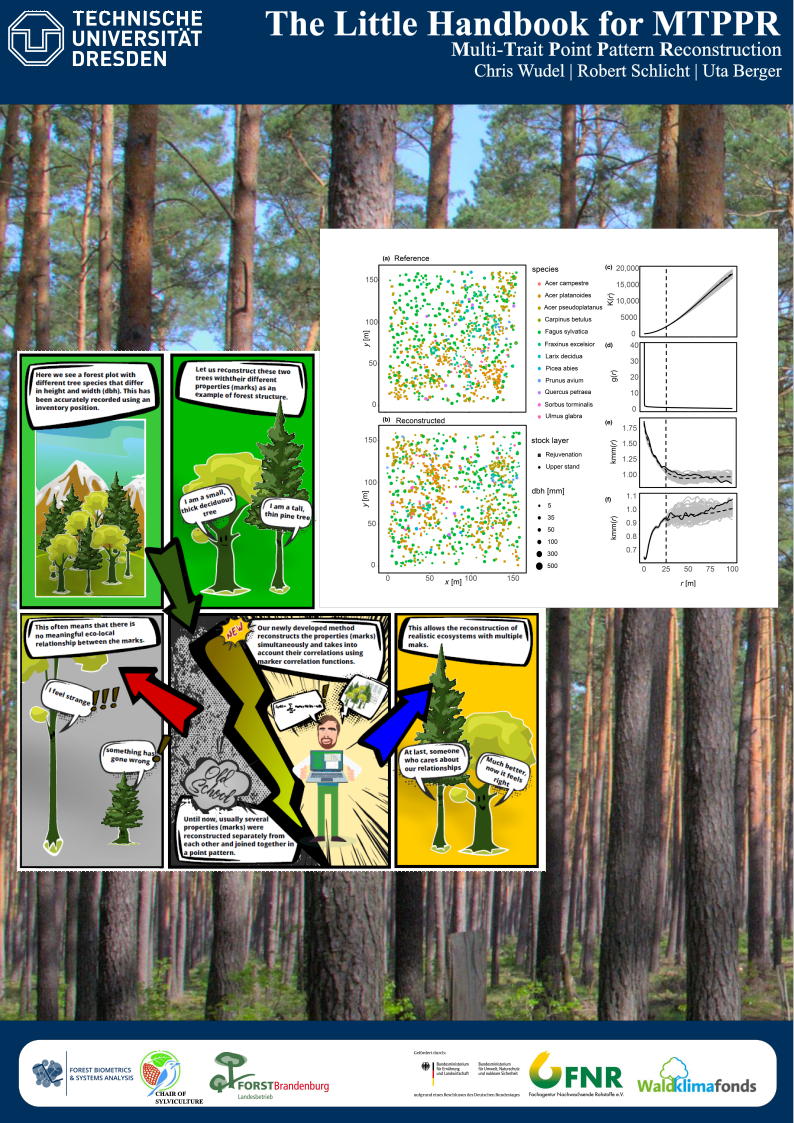
\includegraphics[width=4.16667in,height=\textheight]{images/cover.png}
\end{center}

\bookmarksetup{startatroot}

\chapter{Introduction}\label{introduction}

\textbf{M}ulti-\textbf{T}rait \textbf{P}oint \textbf{P}attern
\textbf{R}econstruction (MTPPR) is a statistical method used to analyze
and reconstruct spatial patterns. Unlike traditional methods, MTPPR
enables the reconstruction of spatial point distributions while
considering multiple associated traits (marks). Previous methods for
reconstructing point patterns either only consider a single mark or
multiple marks independently, neglecting their correlations. MTPPR
employs various second-order summary statistics of point pattern
analysis, such as the pair correlation function and the mark correlation
function.

\textbf{\emph{Figure:}} \emph{This illustration depicts the issue in
reconstructing dot patterns where the correlations between the marks are
not considered. This results in unrealistic proportions, as illustrated
here by the disproportionate trees.}

\begin{center}
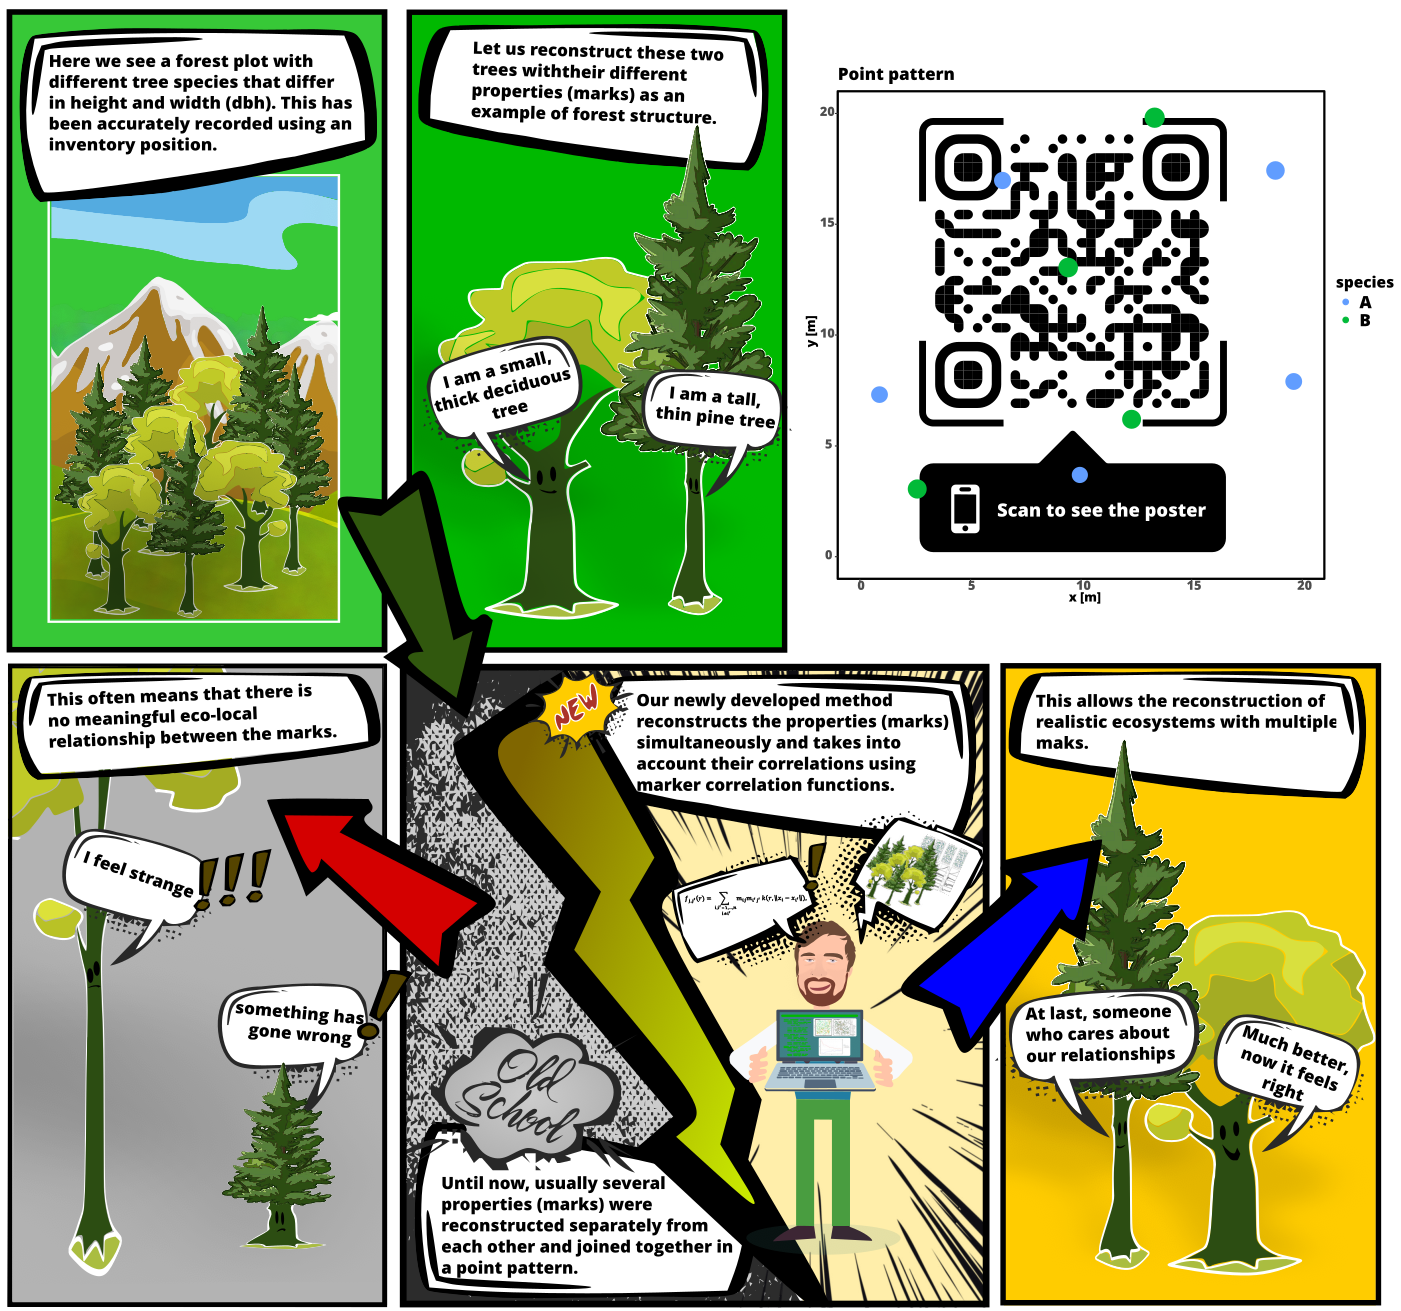
\includegraphics[width=10.41667in,height=\textheight]{images/comic.png}
\end{center}

This method is crucial in fields like ecology, biology, and geography,
where understanding the spatial distribution of entities and their
traits is essential. By considering both the spatial locations and the
various traits of points, MTPPR allows researchers to uncover complex
interactions and dependencies that influence the arrangement and
dynamics of the systems under study.

For example, in ecology, MTPPR can be used to reconstruct the
distribution of different tree species in a forest, taking into account
attributes such as age, height, and health status. This provides
insights into ecological processes such as competition, habitat
preferences, and the impact of environmental factors. Similarly, in
epidemiology, MTPPR can help understand the spread of diseases by
correlating spatial data with demographic and environmental traits.

\subsubsection*{Key Concepts}\label{key-concepts}
\addcontentsline{toc}{subsubsection}{Key Concepts}

\begin{enumerate}
\def\labelenumi{\arabic{enumi}.}
\item
  \textbf{Point Patterns}:

  \begin{itemize}
  \item
    Spatial data points representing the positions of objects or events
    within a defined area.
  \item
    Examples: Locations of trees in a forest, distribution of animal
    burrows, spread of disease cases.
  \end{itemize}
\item
  \textbf{Traits}:

  \begin{itemize}
  \item
    Additional attributes or characteristics associated with each point.
  \item
    Examples: Tree species, age, height, health status.
  \end{itemize}
\item
  \textbf{Multi-Trait Analysis}:

  \begin{itemize}
  \item
    Simultaneous consideration of multiple attributes to understand
    their influence on spatial arrangement.
  \item
    Can reveal complex interactions and dependencies between traits.
  \end{itemize}
\item
  \textbf{Reconstruction}:

  \begin{itemize}
  \item
    Generation of statistically similar point patterns for various
    applications through reconstruction algorithms.
  \item
    Examples: Creating null model patterns for spatial point pattern
    analysis and constructing artificial datasets suitable for
    initializing forest ABMs and other stand simulators.
  \end{itemize}
\end{enumerate}

\subsubsection*{Steps in MTPPR}\label{steps-in-mtppr}
\addcontentsline{toc}{subsubsection}{Steps in MTPPR}

\begin{enumerate}
\def\labelenumi{\arabic{enumi}.}
\item
  \textbf{Data Collection}:

  \begin{itemize}
  \tightlist
  \item
    Gathering spatial data along with associated traits through field
    surveys, remote sensing, or other methods.
  \end{itemize}
\item
  \textbf{Spatial Analysis}:

  \begin{itemize}
  \item
    Analyzing the spatial arrangement of points using techniques such as
    Ripley's K-function, pair correlation function, or spatial
    autocorrelation.
  \item
    Assessing the distribution (clustered, random, regular) and the
    influence of spatial scale.
  \end{itemize}
\item
  \textbf{Trait Analysis}:

  \begin{itemize}
  \tightlist
  \item
    Evaluating the distribution and correlation of traits using methods
    like the mark correlation function.
  \end{itemize}
\item
  \textbf{Model Construction}:

  \begin{itemize}
  \item
    Developing models that integrate spatial and trait information using
    statistical models (e.g., spatial point process models).
  \item
    Aim: Reconstructing the underlying processes leading to the observed
    multi-trait point pattern.
  \end{itemize}
\item
  \textbf{Reconstruction and Validation}:

  \begin{itemize}
  \item
    Reconstructing point patterns based on the developed models to
    predict spatial arrangements under various scenarios.
  \item
    Validating models by comparing simulated patterns with actual
    observations.
  \end{itemize}
\item
  \textbf{Interpretation}:

  \begin{itemize}
  \tightlist
  \item
    Interpreting results to gain insights into ecological, biological,
    or geographical processes.
  \end{itemize}
\end{enumerate}

\subsubsection*{Applications}\label{applications}
\addcontentsline{toc}{subsubsection}{Applications}

\begin{itemize}
\item
  \textbf{Ecology}:

  \begin{itemize}
  \item
    Generating realistic and statistically similar spatial patterns.
  \item
    Understanding the coexistence and competition among plant species.
  \item
    Studying the spatial distribution of animal populations and their
    habitat preferences.
  \end{itemize}
\item
  \textbf{Epidemiology}:

  \begin{itemize}
  \tightlist
  \item
    Analyzing the spread of diseases based on environmental factors and
    population characteristics.
  \end{itemize}
\item
  \textbf{Urban Planning}:

  \begin{itemize}
  \tightlist
  \item
    Assessing the spatial distribution of urban features (e.g., green
    spaces, buildings) and their associated traits (e.g., building
    types, land use).
  \end{itemize}
\end{itemize}

\bookmarksetup{startatroot}

\chapter{Simple application example}\label{simple-application-example}

The following example demonstrates a simple application of
\textbf{M}ulti-\textbf{T}rait \textbf{P}oint \textbf{P}attern
\textbf{R}econstruction (MTPPR) by Wudel et al.~(2023). It illustrates
reconstruction using fictitious datasets that incorporate multiple
traits simultaneously. The required libraries must be loaded beforehand.

\begin{Shaded}
\begin{Highlighting}[]
\FunctionTok{source}\NormalTok{(}\StringTok{"https://raw.githubusercontent.com/ChrisWudel/Multi{-}trait{-}point{-}pattern{-}reconstruction/main/func/reconstruct\_pattern\_multi.R"}\NormalTok{)}
\FunctionTok{source}\NormalTok{(}\StringTok{"https://raw.githubusercontent.com/ChrisWudel/Multi{-}trait{-}point{-}pattern{-}reconstruction/main/func/compute\_statistics.R"}\NormalTok{)}
\FunctionTok{source}\NormalTok{(}\StringTok{"https://raw.githubusercontent.com/ChrisWudel/Multi{-}trait{-}point{-}pattern{-}reconstruction/main/func/dummy\_transf.R"}\NormalTok{)}
\FunctionTok{source}\NormalTok{(}\StringTok{"https://raw.githubusercontent.com/ChrisWudel/Multi{-}trait{-}point{-}pattern{-}reconstruction/main/func/energy\_fun.R"}\NormalTok{)}
\FunctionTok{source}\NormalTok{(}\StringTok{"https://raw.githubusercontent.com/ChrisWudel/Multi{-}trait{-}point{-}pattern{-}reconstruction/main/func/calc\_moments.R"}\NormalTok{)}
\FunctionTok{source}\NormalTok{(}\StringTok{"https://raw.githubusercontent.com/ChrisWudel/Multi{-}trait{-}point{-}pattern{-}reconstruction/main/func/select\_kernel.R"}\NormalTok{)}
\FunctionTok{source}\NormalTok{(}\StringTok{"https://raw.githubusercontent.com/ChrisWudel/Multi{-}trait{-}point{-}pattern{-}reconstruction/main/func/plot.rd\_multi.R"}\NormalTok{)}
\FunctionTok{source}\NormalTok{(}\StringTok{"https://raw.githubusercontent.com/ChrisWudel/Multi{-}trait{-}point{-}pattern{-}reconstruction/main/func/sample\_points.R"}\NormalTok{)}
\FunctionTok{library}\NormalTok{(spatstat)}
\end{Highlighting}
\end{Shaded}

Please note that the maximum number of iterations has been set to
\emph{max\_steps = 10000} and \emph{n\_repetitions = 3} in this example
to keep computation time low. No weighting of different summary
statistics has been performed, which may be necessary for different
applications (e.g., forest stands) to achieve optimal results. For
real-world applications, it is advisable to adjust these parameters
accordingly. Additionally, in the vignette, \emph{verbose = FALSE} has
been set to minimize print output. We recommend using the default
setting verbose = TRUE when running the code to see progress reports.

The next step is to load the point pattern, here is an example of a
random point pattern with several marks to show the structure of the
data used.

\begin{Shaded}
\begin{Highlighting}[]
\NormalTok{xr }\OtherTok{\textless{}{-}} \DecValTok{500}
\NormalTok{yr }\OtherTok{\textless{}{-}} \DecValTok{1000}
\NormalTok{N  }\OtherTok{\textless{}{-}} \DecValTok{400}
\NormalTok{y  }\OtherTok{\textless{}{-}} \FunctionTok{runif}\NormalTok{(N, }\AttributeTok{min =} \DecValTok{0}\NormalTok{, }\AttributeTok{max =}\NormalTok{ yr)}
\NormalTok{x  }\OtherTok{\textless{}{-}} \FunctionTok{runif}\NormalTok{(N, }\AttributeTok{min =} \DecValTok{0}\NormalTok{, }\AttributeTok{max =}\NormalTok{ xr)}
\NormalTok{species  }\OtherTok{\textless{}{-}} \FunctionTok{sample}\NormalTok{(}\FunctionTok{c}\NormalTok{(}\StringTok{"A"}\NormalTok{,}\StringTok{"B"}\NormalTok{), N, }\AttributeTok{replace =} \ConstantTok{TRUE}\NormalTok{)}
\NormalTok{diameter }\OtherTok{\textless{}{-}} \FunctionTok{runif}\NormalTok{(N, }\FloatTok{0.1}\NormalTok{, }\FloatTok{0.4}\NormalTok{)}
\NormalTok{random   }\OtherTok{\textless{}{-}} \FunctionTok{data.frame}\NormalTok{(}\AttributeTok{x =}\NormalTok{ x, }\AttributeTok{y =}\NormalTok{ y, }\AttributeTok{dbh =}\NormalTok{ diameter, }\AttributeTok{species =} \FunctionTok{factor}\NormalTok{(species))}
\NormalTok{marked\_pattern }\OtherTok{\textless{}{-}} \FunctionTok{as.ppp}\NormalTok{(random, }\AttributeTok{W =} \FunctionTok{owin}\NormalTok{(}\FunctionTok{c}\NormalTok{(}\DecValTok{0}\NormalTok{, xr), }\FunctionTok{c}\NormalTok{(}\DecValTok{0}\NormalTok{, yr)))}
\end{Highlighting}
\end{Shaded}

The point pattern must contain the following data An x and y coordinate,
a metric mark (in metres) and a nominal mark defined as a factor. The
order must be respected. Now the reconstruction with several marks can
be started with the following code. Note that the maximum number of
iterations has been set to \emph{max\_steps = 10000} to keep the
computation time for this example to a minimum. For an application, this
value should be increased according to the number of points in the
pattern.

\begin{Shaded}
\begin{Highlighting}[]
\NormalTok{reconstruction }\OtherTok{\textless{}{-}} \FunctionTok{reconstruct\_pattern\_multi}\NormalTok{(marked\_pattern, }\AttributeTok{n\_repetitions =} \DecValTok{1}\NormalTok{, }\AttributeTok{max\_steps =} \DecValTok{10000}\NormalTok{, }\AttributeTok{issue =} \DecValTok{5000}\NormalTok{, }\AttributeTok{verbose =} \ConstantTok{TRUE}\NormalTok{)}
\end{Highlighting}
\end{Shaded}

\begin{verbatim}

> Progress:  || iterations: 0 || Simulation progress: 0% || energy = 0.0594 || energy improvement = 0
> Progress:  || iterations: 5000 || Simulation progress: 50% || energy = 0.00289 || energy improvement = 341
> Progress:  || iterations: 10000 || Simulation progress: 100% || energy = 0.00283 || energy improvement = 547
\end{verbatim}

As a result, you will receive a list containing a variety of
information, for example, the reference pattern, the reconstructed
pattern, the number of successful actions, the energy development and
much more. If you wish to perform several reconstructions of the same
reference pattern, you must increase n\_repetitions to the desired
number.

\begin{Shaded}
\begin{Highlighting}[]
\NormalTok{reconstruction\_2 }\OtherTok{\textless{}{-}} \FunctionTok{reconstruct\_pattern\_multi}\NormalTok{(marked\_pattern, }\AttributeTok{n\_repetitions =} \DecValTok{2}\NormalTok{, }\AttributeTok{max\_steps =} \DecValTok{10000}\NormalTok{, }\AttributeTok{issue =} \DecValTok{5000}\NormalTok{, }\AttributeTok{verbose =} \ConstantTok{TRUE}\NormalTok{)}
\end{Highlighting}
\end{Shaded}

\begin{verbatim}

> Progress: reconstruction_1 || iterations: 0 || Simulation progress: 0% || energy = 0.07468 || energy improvement = 0
> Progress: reconstruction_1 || iterations: 5000 || Simulation progress: 50% || energy = 0.00275 || energy improvement = 387
> Progress: reconstruction_1 || iterations: 10000 || Simulation progress: 100% || energy = 0.00269 || energy improvement = 570


> Progress: reconstruction_2 || iterations: 0 || Simulation progress: 0% || energy = 0.04211 || energy improvement = 0
> Progress: reconstruction_2 || iterations: 5000 || Simulation progress: 50% || energy = 0.00245 || energy improvement = 320
> Progress: reconstruction_2 || iterations: 10000 || Simulation progress: 100% || energy = 0.00239 || energy improvement = 495
\end{verbatim}

To activate a visualisation of the reconstruction that shows the changes
in the pattern at the relevant time, you must proceed as follows.

\begin{Shaded}
\begin{Highlighting}[]
\NormalTok{reconstruction\_3 }\OtherTok{\textless{}{-}} \FunctionTok{reconstruct\_pattern\_multi}\NormalTok{(marked\_pattern, }\AttributeTok{n\_repetitions =} \DecValTok{1}\NormalTok{, }\AttributeTok{max\_steps =} \DecValTok{10000}\NormalTok{, }\AttributeTok{show\_graphic =} \ConstantTok{TRUE}\NormalTok{, }\AttributeTok{issue =} \DecValTok{5000}\NormalTok{, }\AttributeTok{verbose =} \ConstantTok{TRUE}\NormalTok{) }
\end{Highlighting}
\end{Shaded}

\begin{verbatim}

> Progress:  || iterations: 0 || Simulation progress: 0% || energy = 0.06791 || energy improvement = 0
> Progress:  || iterations: 5000 || Simulation progress: 50% || energy = 0.00279 || energy improvement = 316
> Progress:  || iterations: 10000 || Simulation progress: 100% || energy = 0.00277 || energy improvement = 492
\end{verbatim}

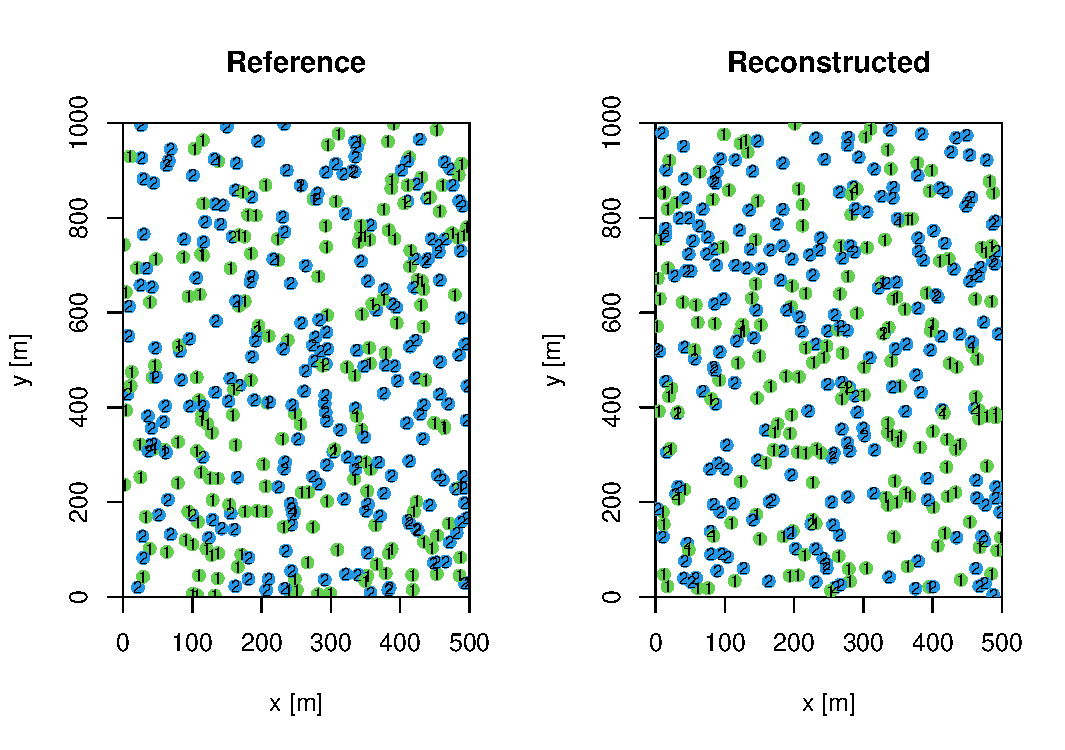
\includegraphics{simple_application_example_files/figure-pdf/unnamed-chunk-5-1.pdf}

Finally, you can use the following function to view different summary
statistics of the reference pattern (black line) compared to the
reconstructed pattern (grey line). For this, however, the listed
libraries must be loaded additionally.

\begin{Shaded}
\begin{Highlighting}[]
\FunctionTok{plot}\NormalTok{(reconstruction)}
\end{Highlighting}
\end{Shaded}

\begin{verbatim}
Progress in the creation of the figures: 100% 
\end{verbatim}

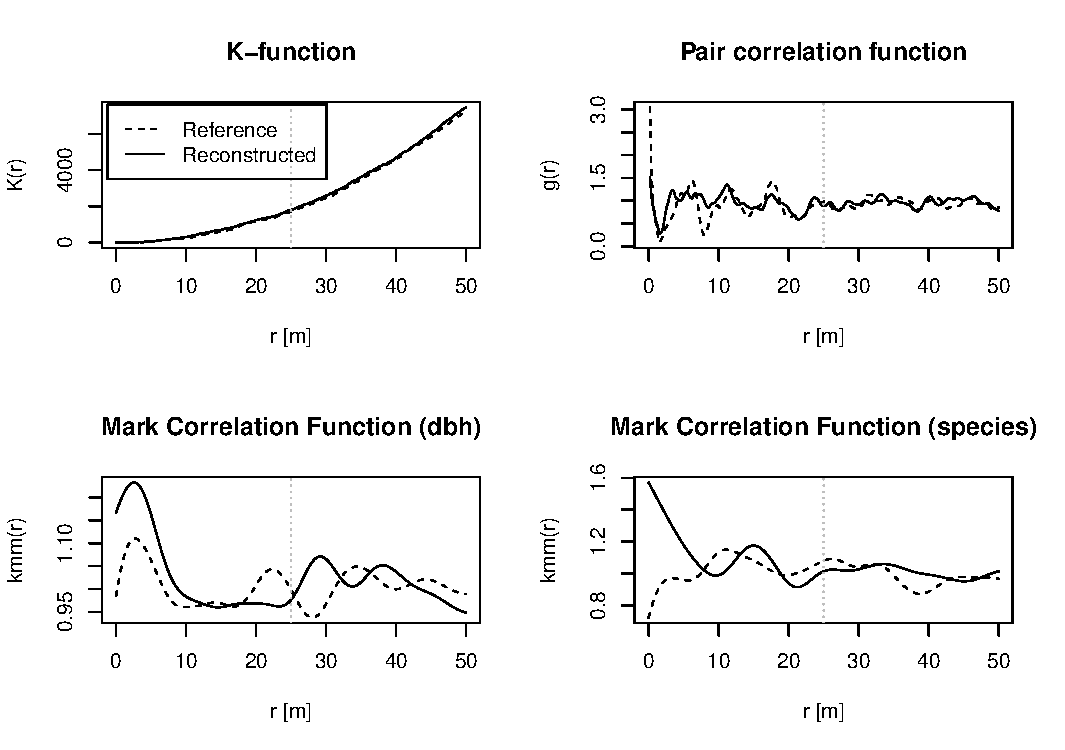
\includegraphics{simple_application_example_files/figure-pdf/unnamed-chunk-6-1.pdf}

\bookmarksetup{startatroot}

\chapter{Further application
examples}\label{further-application-examples}

In the following, further examples of the simple application of
\textbf{M}ulti-\textbf{T}rait \textbf{P}oint \textbf{P}attern
\textbf{R}econstruction (MTPPR) by Wudel et al.~(2023) are presented.
These are standard applications, meaning that reconstructions are
performed without enlargements or reductions of the reconstruction
pattern and without edge correction.

First, the necessary functions and packages will be loaded. If
individual R packages are not installed, install them as follows:
\texttt{install.packages("package\ name")}.

\begin{Shaded}
\begin{Highlighting}[]
\FunctionTok{source}\NormalTok{(}\StringTok{"https://raw.githubusercontent.com/ChrisWudel/Multi{-}trait{-}point{-}pattern{-}reconstruction/main/func/reconstruct\_pattern\_multi.R"}\NormalTok{)}
\FunctionTok{source}\NormalTok{(}\StringTok{"https://raw.githubusercontent.com/ChrisWudel/Multi{-}trait{-}point{-}pattern{-}reconstruction/main/func/compute\_statistics.R"}\NormalTok{)}
\FunctionTok{source}\NormalTok{(}\StringTok{"https://raw.githubusercontent.com/ChrisWudel/Multi{-}trait{-}point{-}pattern{-}reconstruction/main/func/dummy\_transf.R"}\NormalTok{)}
\FunctionTok{source}\NormalTok{(}\StringTok{"https://raw.githubusercontent.com/ChrisWudel/Multi{-}trait{-}point{-}pattern{-}reconstruction/main/func/energy\_fun.R"}\NormalTok{)}
\FunctionTok{source}\NormalTok{(}\StringTok{"https://raw.githubusercontent.com/ChrisWudel/Multi{-}trait{-}point{-}pattern{-}reconstruction/main/func/calc\_moments.R"}\NormalTok{)}
\FunctionTok{source}\NormalTok{(}\StringTok{"https://raw.githubusercontent.com/ChrisWudel/Multi{-}trait{-}point{-}pattern{-}reconstruction/main/func/select\_kernel.R"}\NormalTok{)}
\FunctionTok{source}\NormalTok{(}\StringTok{"https://raw.githubusercontent.com/ChrisWudel/Multi{-}trait{-}point{-}pattern{-}reconstruction/main/func/plot.rd\_multi.R"}\NormalTok{)}
\FunctionTok{source}\NormalTok{(}\StringTok{"https://raw.githubusercontent.com/ChrisWudel/Multi{-}trait{-}point{-}pattern{-}reconstruction/main/func/sample\_points.R"}\NormalTok{)}

\FunctionTok{source}\NormalTok{(}\StringTok{"https://raw.githubusercontent.com/ChrisWudel/Multi{-}trait{-}point{-}pattern{-}reconstruction/main/func/vis\_patterns.R"}\NormalTok{)}
\FunctionTok{source}\NormalTok{(}\StringTok{"https://raw.githubusercontent.com/ChrisWudel/Multi{-}trait{-}point{-}pattern{-}reconstruction/main/func/select\_data.R"}\NormalTok{)}

\FunctionTok{library}\NormalTok{(spatstat)}
\FunctionTok{library}\NormalTok{(ggplot2)}
\FunctionTok{library}\NormalTok{(patchwork)}
\end{Highlighting}
\end{Shaded}

Now you need to define which dataset you want to use. There are 2 real
datasets and 4 generated datasets available. To select a dataset, define
\emph{x} with the name of the dataset you want to use (\emph{x
\textless- `Dataset Name'}). The datasets are available under 'Records
for download.

\begin{Shaded}
\begin{Highlighting}[]
\NormalTok{x }\OtherTok{\textless{}{-}} \StringTok{"random"} \DocumentationTok{\#\# The following sets can be imported: }
                                   \DocumentationTok{\#\# Real datasets:}
                                    \DocumentationTok{\#\#    "VERMOS\_project" }
                                    \DocumentationTok{\#\#    "Northwest\_German\_Forest\_Research\_Institute" }
                                    \DocumentationTok{\#\#   "Marteloscope\_data\_from\_the\_by\_the\_Chair\_of\_Forest\_Growth\_and\_Woody\_Biomass\_Production"}
                                   \DocumentationTok{\#\# Simulated patterns:}
                                    \DocumentationTok{\#\#    "random"}
                                    \DocumentationTok{\#\#    "regular"}
                                    \DocumentationTok{\#\#    "cluster\_size5"}
                                    \DocumentationTok{\#\#    "cluster\_size5\_and\_random"}
                                   \DocumentationTok{\#\# to do this, declare x with the corresponding name in "". }
\NormalTok{data }\OtherTok{\textless{}{-}} \FunctionTok{data\_import}\NormalTok{(x)}
\NormalTok{W }\OtherTok{\textless{}{-}}\NormalTok{ data[[}\DecValTok{2}\NormalTok{]] }
\NormalTok{data }\OtherTok{\textless{}{-}}\NormalTok{ data [[}\DecValTok{1}\NormalTok{]] }
\end{Highlighting}
\end{Shaded}

The following parameters are predefined and can be varied arbitrarily in
an application file (Application of the Multi-trait Point pattern
reconstruction.R) where you can use this code, available for download
under the Application folder. It should be noted that for optimal
results, the parameter max\_steps should be at least approximately ten
times the number of points in the pattern, and the parameter for weights
(w\_markcorr) of individual summary statistics needs to be adjusted
according to different scenarios. Here, a small number of steps was
chosen to save computation time.

\begin{Shaded}
\begin{Highlighting}[]
\NormalTok{marked\_pattern }\OtherTok{\textless{}{-}} \FunctionTok{as.ppp}\NormalTok{(}\FunctionTok{data.frame}\NormalTok{(data), }\AttributeTok{W =}\NormalTok{ W)   }
\NormalTok{marked\_pattern}\SpecialCharTok{$}\NormalTok{marks}\SpecialCharTok{$}\NormalTok{dbh..mm.}\OtherTok{\textless{}{-}}\NormalTok{marked\_pattern}\SpecialCharTok{$}\NormalTok{marks}\SpecialCharTok{$}\NormalTok{dbh..mm.}\SpecialCharTok{*}\FloatTok{0.001}   
\NormalTok{xr }\OtherTok{\textless{}{-}}\NormalTok{ marked\_pattern}\SpecialCharTok{$}\NormalTok{window}\SpecialCharTok{$}\NormalTok{xrange}
\NormalTok{yr }\OtherTok{\textless{}{-}}\NormalTok{ marked\_pattern}\SpecialCharTok{$}\NormalTok{window}\SpecialCharTok{$}\NormalTok{yrange}
                                                                               
\NormalTok{reconstruction }\OtherTok{\textless{}{-}} \FunctionTok{reconstruct\_pattern\_multi}\NormalTok{(}
\NormalTok{  marked\_pattern, }
  \AttributeTok{n\_repetitions     =} \DecValTok{1}\NormalTok{,     }
  \AttributeTok{max\_steps         =} \DecValTok{10000}\NormalTok{,     }
  \AttributeTok{no\_change         =} \DecValTok{5}\NormalTok{,  }
  \AttributeTok{rcount            =} \DecValTok{250}\NormalTok{,     }
  \AttributeTok{rmax              =} \DecValTok{25}\NormalTok{,      }
  \AttributeTok{issue             =} \DecValTok{1000}\NormalTok{,       }
  \AttributeTok{divisor           =} \StringTok{"r"}\NormalTok{,    }
  \AttributeTok{kernel\_arg        =} \StringTok{"epanechnikov"}\NormalTok{,}
  \AttributeTok{timing            =} \ConstantTok{TRUE}\NormalTok{,    }
  \AttributeTok{energy\_evaluation =} \ConstantTok{TRUE}\NormalTok{,}
  \AttributeTok{show\_graphic      =} \ConstantTok{FALSE}\NormalTok{,  }
  \AttributeTok{Lp                =} \DecValTok{1}\NormalTok{,    }
  \AttributeTok{bw                =} \FloatTok{0.5}\NormalTok{,}
  \AttributeTok{sd                =} \StringTok{"step"}\NormalTok{,}
  \AttributeTok{steps\_tol         =} \DecValTok{1000}\NormalTok{,   }
  \AttributeTok{tol               =} \FloatTok{1e{-}4}\NormalTok{,   }
  \AttributeTok{w\_markcorr        =} \FunctionTok{c}\NormalTok{(}\AttributeTok{m\_m=}\DecValTok{1}\NormalTok{,}\AttributeTok{one\_one=}\DecValTok{0}\NormalTok{,  }\AttributeTok{all=}\DecValTok{1}\NormalTok{, }\AttributeTok{m\_all=}\DecValTok{1}\NormalTok{, }\AttributeTok{all\_all=}\DecValTok{1}\NormalTok{, }\AttributeTok{m\_m0=}\DecValTok{1}\NormalTok{, }\AttributeTok{one\_one0=}\DecValTok{0}\NormalTok{, }\AttributeTok{all0=}\DecValTok{1}\NormalTok{, }\AttributeTok{m\_all0=}\DecValTok{1}\NormalTok{, }\AttributeTok{all\_all0=}\DecValTok{1}\NormalTok{),}
  \AttributeTok{prob\_of\_actions   =} \FunctionTok{c}\NormalTok{(}\AttributeTok{move\_coordinate =} \FloatTok{0.4}\NormalTok{, }\AttributeTok{switch\_coords =} \FloatTok{0.1}\NormalTok{, }\AttributeTok{exchange\_mark\_one =} \FloatTok{0.1}\NormalTok{, }\AttributeTok{exchange\_mark\_two =} \FloatTok{0.1}\NormalTok{, }\AttributeTok{pick\_mark\_one =} \FloatTok{0.2}\NormalTok{, }\AttributeTok{pick\_mark\_two =} \FloatTok{0.1}\NormalTok{, }\AttributeTok{delete\_point =} \FloatTok{0.0}\NormalTok{, }\AttributeTok{add\_point =} \FloatTok{0.0}\NormalTok{), }
  \AttributeTok{k                 =} \DecValTok{1}\NormalTok{,       }
  \AttributeTok{w\_statistics      =} \FunctionTok{c}\NormalTok{(),              }
  \AttributeTok{verbose           =} \ConstantTok{TRUE}\NormalTok{)  }
\end{Highlighting}
\end{Shaded}

As a result, you will receive a list with a variety of information, such
as the reference pattern, the reconstructed pattern, the number of
successful actions, the energy development, and much more. To illustrate
the results, first compare the reference pattern with the reconstructed
pattern.

\begin{Shaded}
\begin{Highlighting}[]
\FunctionTok{vis\_pp}\NormalTok{(reconstruction) }
\end{Highlighting}
\end{Shaded}

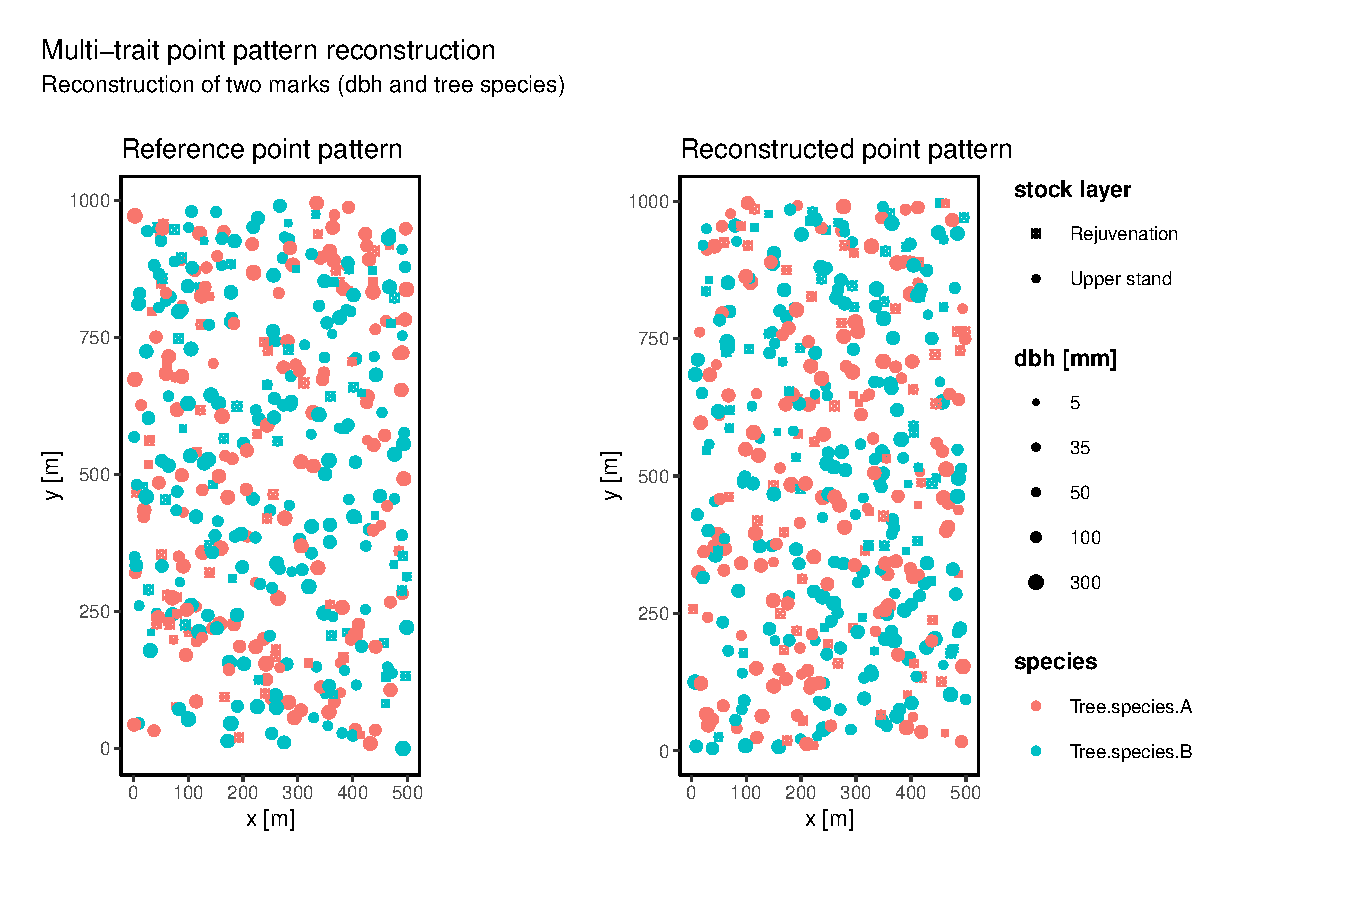
\includegraphics{further_application_examples_files/figure-pdf/unnamed-chunk-4-1.pdf}

Finally, you can use the following function to compare various summary
statistics of the reference pattern (black line) with the reconstructed
pattern (grey line). Another function (plot\_sum\_stat) is capable of
displaying these summary statistics in a single diagram for multiple
repetitions of the reconstructions (n\_repetitions \textgreater{} 1),
and it is used in the previously mentioned application file (Application
of the Multi-trait Point pattern reconstruction.R). For simplicity, this
functionality has been omitted here.

\begin{Shaded}
\begin{Highlighting}[]
\FunctionTok{plot}\NormalTok{(reconstruction)}
\end{Highlighting}
\end{Shaded}

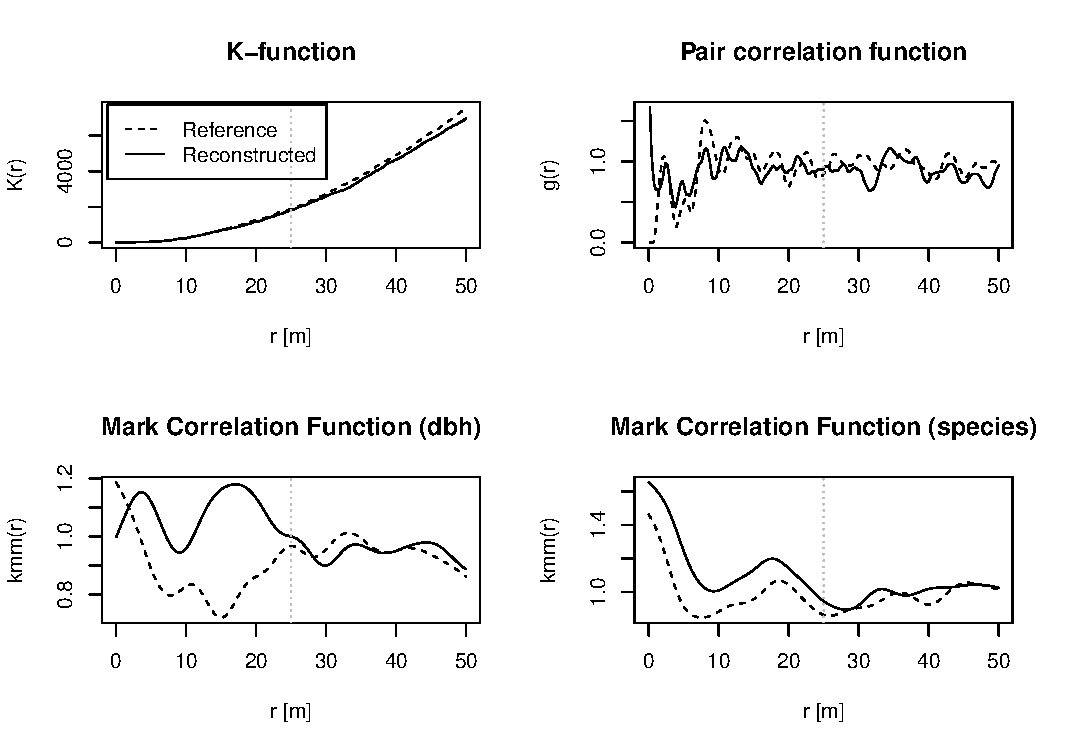
\includegraphics{further_application_examples_files/figure-pdf/unnamed-chunk-5-1.pdf}

\bookmarksetup{startatroot}

\chapter{Specialized application}\label{specialized-application}

This represents \textbf{a novel workflow for predicting forest
regeneration}. Initially, the canopy of a forest area and a small
portion of the regeneration were captured using terrestrial laser
scanning. Based on spatial statistical tree data and correlations
between tree characteristics, a point pattern reconstruction method was
developed, building upon the work of Wudel et al.~(2023). This method
facilitates the prediction of regeneration across the entire area with
high accuracy.

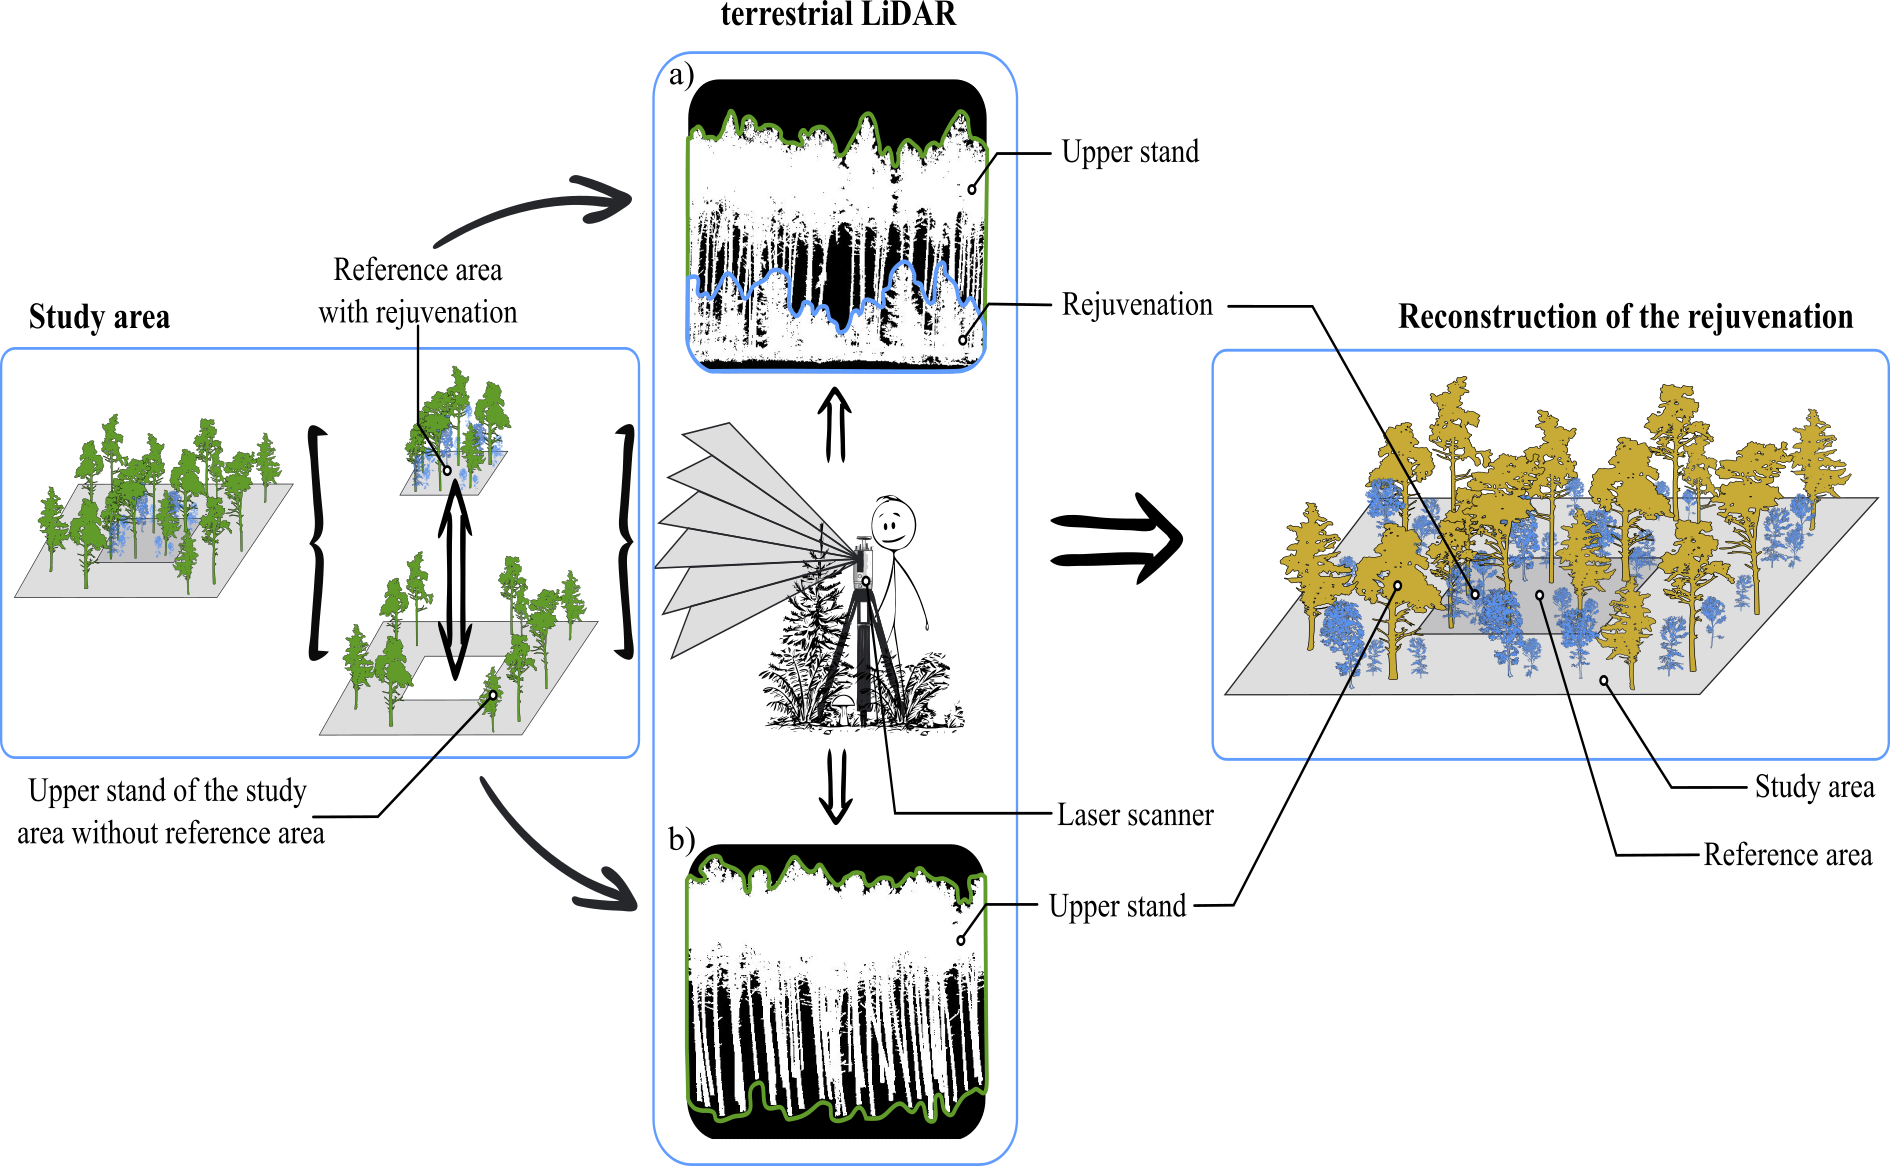
\includegraphics{workflow.png}

\emph{\textbf{Figure:} Conceptual presentation of the new innovative
workflow for data acquisition and reconstruction of forest regeneration
(LiDAR = Light Detection and Ranging). a) Recording regeneration on a
small area and b) recording of the upper stand trees at the whole forest
area.}

The following code can be used to execute the workflow using an
available dataset. First, the necessary functions and packages are
loaded.

\begin{Shaded}
\begin{Highlighting}[]
\FunctionTok{source}\NormalTok{(}\StringTok{"https://raw.githubusercontent.com/ChrisWudel/Multi{-}trait{-}point{-}pattern{-}reconstruction/main/func/reconstruct\_pattern\_multi.R"}\NormalTok{)}
\FunctionTok{source}\NormalTok{(}\StringTok{"https://raw.githubusercontent.com/ChrisWudel/Multi{-}trait{-}point{-}pattern{-}reconstruction/main/func/compute\_statistics.R"}\NormalTok{)}
\FunctionTok{source}\NormalTok{(}\StringTok{"https://raw.githubusercontent.com/ChrisWudel/Multi{-}trait{-}point{-}pattern{-}reconstruction/main/func/dummy\_transf.R"}\NormalTok{)}
\FunctionTok{source}\NormalTok{(}\StringTok{"https://raw.githubusercontent.com/ChrisWudel/Multi{-}trait{-}point{-}pattern{-}reconstruction/main/func/energy\_fun.R"}\NormalTok{)}
\FunctionTok{source}\NormalTok{(}\StringTok{"https://raw.githubusercontent.com/ChrisWudel/Multi{-}trait{-}point{-}pattern{-}reconstruction/main/func/calc\_moments.R"}\NormalTok{)}
\FunctionTok{source}\NormalTok{(}\StringTok{"https://raw.githubusercontent.com/ChrisWudel/Multi{-}trait{-}point{-}pattern{-}reconstruction/main/func/select\_kernel.R"}\NormalTok{)}
\FunctionTok{source}\NormalTok{(}\StringTok{"https://raw.githubusercontent.com/ChrisWudel/Multi{-}trait{-}point{-}pattern{-}reconstruction/main/func/plot.rd\_multi.R"}\NormalTok{)}
\FunctionTok{source}\NormalTok{(}\StringTok{"https://raw.githubusercontent.com/ChrisWudel/Multi{-}trait{-}point{-}pattern{-}reconstruction/main/func/sample\_points.R"}\NormalTok{)}
\FunctionTok{source}\NormalTok{(}\StringTok{"https://raw.githubusercontent.com/ChrisWudel/Multi{-}trait{-}point{-}pattern{-}reconstruction/main/func/edge\_correction.R"}\NormalTok{)}

\FunctionTok{source}\NormalTok{(}\StringTok{"https://raw.githubusercontent.com/ChrisWudel/Multi{-}trait{-}point{-}pattern{-}reconstruction/main/func/vis\_patterns.R"}\NormalTok{)}

\FunctionTok{library}\NormalTok{(spatstat)}
\FunctionTok{library}\NormalTok{(ggplot2)}
\end{Highlighting}
\end{Shaded}

Anschlißende wird der Datensatz aufgerfen der in Github im Orner Records
zu finden ist und published and freely available at the following link:
\url{https://zenodo.org/records/10550778} (Meyer and Wudel, 2024).

\begin{Shaded}
\begin{Highlighting}[]
\NormalTok{url }\OtherTok{\textless{}{-}}\StringTok{"C:/Users/admin/Desktop/New Paper/step{-}by{-}step application/Data/TLS\_core.csv"}
\NormalTok{data }\OtherTok{\textless{}{-}} \FunctionTok{read.csv}\NormalTok{(url,}\AttributeTok{sep =} \StringTok{","}\NormalTok{, }\AttributeTok{stringsAsFactors=} \ConstantTok{TRUE}\NormalTok{)}
\NormalTok{data}\SpecialCharTok{$}\NormalTok{dbh }\OtherTok{\textless{}{-}} \FunctionTok{as.numeric}\NormalTok{(data}\SpecialCharTok{$}\NormalTok{dbh)}
\end{Highlighting}
\end{Shaded}

Below are the parameter settings chosen for this example. These may and
should be adjusted for other datasets to achieve good results. Note: the
maximum number of steps has also been reduced here to limit computation
time.

\begin{Shaded}
\begin{Highlighting}[]
\NormalTok{W }\OtherTok{\textless{}{-}} \FunctionTok{owin}\NormalTok{(}\FunctionTok{c}\NormalTok{(}\DecValTok{0}\NormalTok{, }\DecValTok{100}\NormalTok{),}\FunctionTok{c}\NormalTok{(}\DecValTok{0}\NormalTok{, }\DecValTok{100}\NormalTok{))}
\NormalTok{core\_window }\OtherTok{\textless{}{-}} \FunctionTok{owin}\NormalTok{(}\FunctionTok{c}\NormalTok{(}\DecValTok{35}\NormalTok{, }\DecValTok{65}\NormalTok{),}\FunctionTok{c}\NormalTok{(}\DecValTok{35}\NormalTok{, }\DecValTok{65}\NormalTok{))}

\NormalTok{marked\_pattern }\OtherTok{\textless{}{-}} \FunctionTok{as.ppp}\NormalTok{(}\FunctionTok{data.frame}\NormalTok{(data), }\AttributeTok{W =}\NormalTok{ W)  }
\NormalTok{marked\_pattern}\SpecialCharTok{$}\NormalTok{marks}\SpecialCharTok{$}\NormalTok{dbh }\OtherTok{\textless{}{-}}\NormalTok{ marked\_pattern}\SpecialCharTok{$}\NormalTok{marks}\SpecialCharTok{$}\NormalTok{dbh}\SpecialCharTok{*}\FloatTok{0.001}  
\NormalTok{xr }\OtherTok{\textless{}{-}}\NormalTok{ marked\_pattern}\SpecialCharTok{$}\NormalTok{window}\SpecialCharTok{$}\NormalTok{xrange}
\NormalTok{yr }\OtherTok{\textless{}{-}}\NormalTok{ marked\_pattern}\SpecialCharTok{$}\NormalTok{window}\SpecialCharTok{$}\NormalTok{yrange}
\NormalTok{obs\_window }\OtherTok{=} \FunctionTok{owin}\NormalTok{(}\FunctionTok{c}\NormalTok{(xr),}\FunctionTok{c}\NormalTok{(yr))}

\NormalTok{reconstruction }\OtherTok{\textless{}{-}} \FunctionTok{reconstruct\_pattern\_multi}\NormalTok{(}
\NormalTok{marked\_pattern,}
\AttributeTok{fixed\_points      =} \ConstantTok{NULL}\NormalTok{,}
\AttributeTok{edge\_correction   =} \ConstantTok{TRUE}\NormalTok{,     }
\AttributeTok{n\_repetitions     =} \DecValTok{1}\NormalTok{,     }
\AttributeTok{max\_steps         =} \DecValTok{10000}\NormalTok{,     }
\AttributeTok{no\_change         =} \DecValTok{5}\NormalTok{,     }
\AttributeTok{rcount            =} \DecValTok{250}\NormalTok{,     }
\AttributeTok{rmax              =} \DecValTok{25}\NormalTok{,      }
\AttributeTok{issue             =} \DecValTok{5000}\NormalTok{,       }
\AttributeTok{divisor           =} \StringTok{"r"}\NormalTok{,    }
\AttributeTok{kernel\_arg        =} \StringTok{"epanechnikov"}\NormalTok{,}
\AttributeTok{timing            =} \ConstantTok{TRUE}\NormalTok{,    }
\AttributeTok{energy\_evaluation =} \ConstantTok{TRUE}\NormalTok{,}
\AttributeTok{show\_graphic      =} \ConstantTok{FALSE}\NormalTok{,  }
\AttributeTok{Lp                =} \DecValTok{1}\NormalTok{,      }
\AttributeTok{bw                =} \FloatTok{0.5}\NormalTok{,}
\AttributeTok{sd                =} \StringTok{"step"}\NormalTok{,}
\AttributeTok{steps\_tol         =} \DecValTok{10000}\NormalTok{,   }
\AttributeTok{tol               =} \FloatTok{1e{-}4}\NormalTok{,   }
\AttributeTok{w\_markcorr        =} \FunctionTok{c}\NormalTok{(}\AttributeTok{m\_m=}\DecValTok{0}\NormalTok{,}\AttributeTok{one\_one=}\DecValTok{1500}\NormalTok{,  }\AttributeTok{all=}\DecValTok{1}\NormalTok{, }\AttributeTok{m\_all=}\DecValTok{1}\NormalTok{, }\AttributeTok{all\_all=}\DecValTok{1}\NormalTok{, }\AttributeTok{m\_m0=}\DecValTok{1500}\NormalTok{, }\AttributeTok{one\_one0=}\DecValTok{1}\NormalTok{, }\AttributeTok{all0=}\DecValTok{1}\NormalTok{, }\AttributeTok{m\_all0=}\DecValTok{1}\NormalTok{, }\AttributeTok{all\_all0=}\DecValTok{1}\NormalTok{),}
\AttributeTok{prob\_of\_actions   =} \FunctionTok{c}\NormalTok{(}\AttributeTok{move\_coordinate =} \FloatTok{0.3}\NormalTok{, }\AttributeTok{switch\_coords =} \FloatTok{0.1}\NormalTok{, }\AttributeTok{exchange\_mark\_one =} \FloatTok{0.1}\NormalTok{, }\AttributeTok{exchange\_mark\_two =} \FloatTok{0.1}\NormalTok{, }\AttributeTok{pick\_mark\_one =} \FloatTok{0.1}\NormalTok{, }\AttributeTok{pick\_mark\_two =} \FloatTok{0.1}\NormalTok{, }\AttributeTok{delete\_point =} \FloatTok{0.1}\NormalTok{, }\AttributeTok{add\_point =} \FloatTok{0.1}\NormalTok{), }
\AttributeTok{k                 =} \DecValTok{1}\NormalTok{,       }
\AttributeTok{w\_statistics      =} \FunctionTok{c}\NormalTok{(),              }
\AttributeTok{is.fixed          =} \ControlFlowTok{function}\NormalTok{(p) }\DecValTok{35} \SpecialCharTok{\textless{}=}\NormalTok{ p}\SpecialCharTok{$}\NormalTok{x }\SpecialCharTok{\&}\NormalTok{ p}\SpecialCharTok{$}\NormalTok{x }\SpecialCharTok{\textless{}=} \DecValTok{65} \SpecialCharTok{\&} \DecValTok{35} \SpecialCharTok{\textless{}=}\NormalTok{ p}\SpecialCharTok{$}\NormalTok{y }\SpecialCharTok{\&}\NormalTok{ p}\SpecialCharTok{$}\NormalTok{y }\SpecialCharTok{\textless{}=} \DecValTok{65} \SpecialCharTok{|}\NormalTok{ p}\SpecialCharTok{$}\NormalTok{mark[,}\StringTok{"dbh"}\NormalTok{] }\SpecialCharTok{\textgreater{}} \FloatTok{0.1}\NormalTok{,}
\AttributeTok{verbose           =} \ConstantTok{TRUE}\NormalTok{) }
\end{Highlighting}
\end{Shaded}

\begin{verbatim}

> Progress:  || iterations: 0 || Simulation progress: 0% || energy = 32913.12269 || energy improvement = 0
> Progress:  || iterations: 5000 || Simulation progress: 50% || energy = 14717.70558 || energy improvement = 56
> Progress:  || iterations: 10000 || Simulation progress: 100% || energy = 4067.98167 || energy improvement = 71
\end{verbatim}

The following figure shows the results of the workflow, which are from
an example not derived from the current run. The figure has been created
retroactively and is not generated by the function provided.
Additionally, in this simulation, significantly more simulation steps
were conducted, which would take too long to render for this handbook.

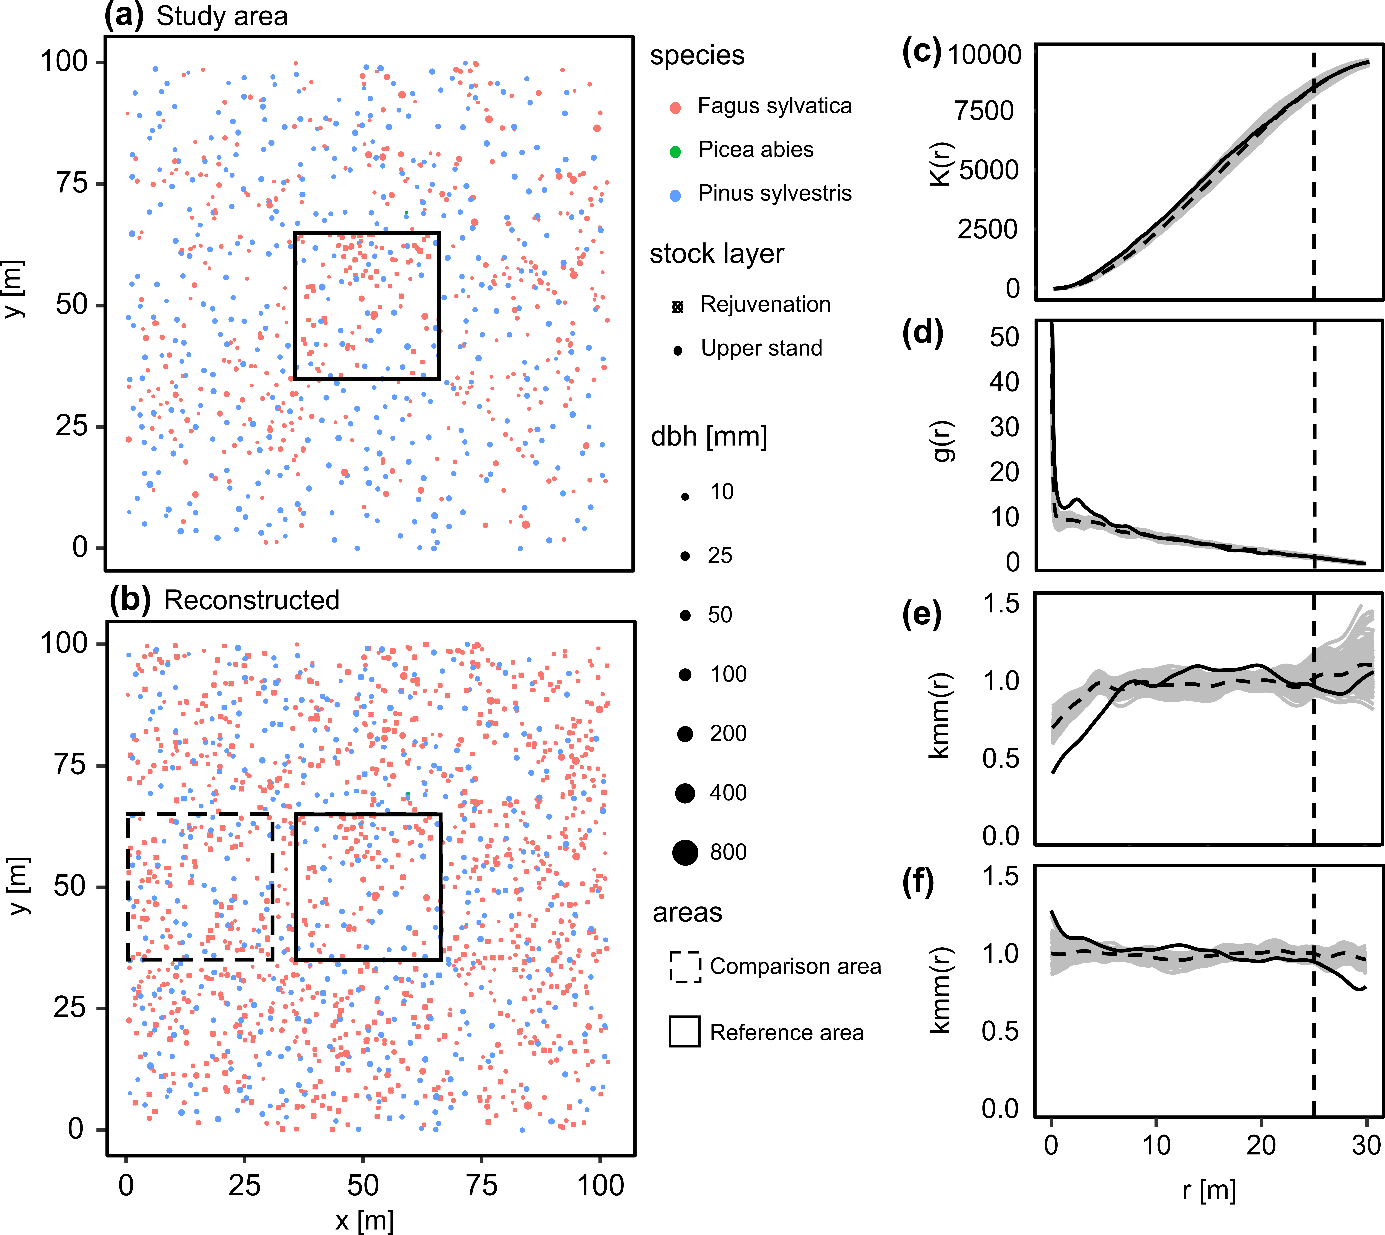
\includegraphics{images/results_TLS.png}

\emph{\textbf{Figure:} Results of the 100 reconstructions of the dataset
described above; (a) reference pattern with core area, black outlined
area (b) an example of a reconstruction in which the core area is
outlined in black and the comparison area is outlined in black dashed
lines. Summary statistics (c)--(f) were generated using the R package
`spatstat': (c) K function; (d) pcf; (e) mcf of the species, where the
test function has value if both species coincide and if not; (f) mcf of
the diameter, the test function being the usual product. For distances
up to  = 25 m (indicated by the vertical dashed line in (c)--(f)). The
black solid lines represent the reference curve and the grey solid lines
represent the 100 reconstructions. The dashed black line is the mean of
the 100 reconstructions.}

It is evident that the tree distributions in these two areas are
similar. For instance, Fagus sylvatica is observed with high intensity
only in specific regions of the reference area, and this has been
successfully reproduced. Furthermore, it is noticeable that smaller gaps
in the reference area, where canopy trees are spaced similarly, are not
occupied by regeneration plants in the comparison area. Also includes
the previously mentioned summary statistics of all 100 reconstructions
(c)-(f). These statistics demonstrate that the reconstructions perform
well (gray lines = reconstructions, solid black line = reference).
Within the range up to 25 m, which was considered during reconstruction,
deviations from the reference in the K-function (c) are minimal. The pcf
(d) shows a slight systematic deviation. The mcf of the species (e)
exhibit only minimal discrepancies. The mcf of diameters (f) show
smaller discrepancies in the same close range as the pcf. However,
deviations become significantly larger and more diverse once the 25 m
range is exceeded. This highlights the effectiveness and impact of the
mcf's in the reconstruction method.

\bookmarksetup{startatroot}

\chapter{Summary and references}\label{summary-and-references}

This Handbook is intended to facilitate the use of MTPPR and to
illustrate its broad application through various examples. The method is
still under development and will be regularly updated with changes.

If you have any questions, please contact the author:

\textbf{Chris Wudel}, Email: \ul{chris.wudel@tu-dresden.de}

Or one of the following co-authors:

\begin{itemize}
\item
  \textbf{Dr.~Robert Schlicht} (co-developer), Email:
  \ul{robert.schlicht@tu-dresden.de}
\item
  \textbf{Prof.~Dr.~Uta Berge}r (supervised and revised), Email:
  \ul{uta.berger@tu-dresden.de}
\item
  \textbf{Dr.~Franka Huth} (data collection and forestry consultation),
  Email: \ul{franka.huth@tu-dresden.de}
\item
  \textbf{Nora Meyer} (data collection TLS), Email:
  \ul{nora.meyer@tu-dresden.de}
\item
  \textbf{Alexandra Wehnert} (data collection), Email:
  \ul{alexandra.wehnert@tu-dresden.de}
\end{itemize}

\bookmarksetup{startatroot}

\chapter*{References}\label{references}
\addcontentsline{toc}{chapter}{References}

\markboth{References}{References}

Further references, for example regarding the method description, can be
found in the respective publications.

\begin{itemize}
\item
  Fichtner, I., van der Maaten-Theunissen, M., 2022. Marteloscope data
  of the experimental plot, Naundorf 710 b1 (Saxony, Germany 2020).
  Zenodo. \url{https://doi.org/10.5281/zenodo.7147868}
\item
  Meyer, N., Wudel, C., 2024. Terrestrial laser scan data of a
  experimental plot in Forstamt Billenhagen, 340 a31 (Mecklenburg-
  Vorpommern, Germany 2023).
  \url{https://doi.org/10.5281/zenodo.10550778}
\item
  Wudel, C., Huth, F., Wehnert, A., 2022a. Individual tree data of the
  temporary test plot Neusorgefeld 5138 - VERMOS project. Zenodo.
  \url{https://doi.org/10.5281/zenodo.7157076}
\item
  Wudel, C., Schlicht, R., Berger, U., 2023. Multi-trait point pattern
  reconstruction of plant ecosystems. Methods Ecol. Evol. 14,
  2668--2679.
  \url{https://doi.org/https://doi.org/10.1111/2041-210X.14206}
\item
  Wudel, C., Schlicht, R., Berger, U., 2022b.
  Point-pattern-reconstruction. Zenodo.
  \url{https://doi.org/10.5281/zenodo.7228767}
\end{itemize}




\end{document}
